\documentclass[a4paper]{efr}

\usepackage{verbatim}
\usepackage{graphicx}
%\usepackage{ctable}
%\usepackage{longtable}
%\usepackage{rotating}
%\usepackage{makecell}

%\bibliographystyle{plain}

\def\fboxsep{5pt}
  \newenvironment{myboxenv}[1]
  {
    \begin{flushright}
      \begin{boxedminipage}{0.9\textwidth}
        \textbf{%% \sffamily
          \large #1:}

        \hspace{-5pt}\rule{0.3\textwidth}{0.5pt}
        \begin{center}
          \begin{minipage}{0.95\textwidth}

            \small%% \slshape
         }
          {
          \end{minipage}
        \end{center}
      \end{boxedminipage}
    \end{flushright}
 }

\title{The Enlightenment Foundation Libraries\\
  \normalsize{Prise en main de Edje}}

\EfrMail{aguirre.nicolas@gmail.com}
\author{Nicolas Aguirre}

\begin{document}

\maketitle
\tableofcontents

\section{Avant Propos}
Le but de ce tutorial est de survoler au travers d'un exemple pratique toutes
les fonctionnalités de Edje.

J'espére qu'il vous permettra également de vous faire comprendre comment Edje
peut vous aider dans le développement de vos interfaces graphiques.

De considerer cette technologie comme l'un des outils les plus puissant des
EFL plutôt que comme votre plus grand cauchemar.

Comment, en séparant la logique et le code d'une part et l'interface d'une
autre, vos interfaces graphiques peuvent gagner en flexibilité.

Comme exemple concret, permettant d'illustrer cette présentation, j'ai choisis
le développement d'un interface (tactile) tres simple.
Voici a quoi ressemblera l'interface a la fin de ce tutoriel :

\section{Introduction}
Edje est une des briques de base des EFL. Elle vous permet de décrire une
interface graphique sans écrire une seule ligne de C. Ce qui permet,de facto,
de réaliser une des choses les plus complexes lors du développement d'un
programme avec une interface utilisateur : la séparation de l'interface et du
code. Cette séparation est importante à plus d'un titre. Elle permet d'une part
d'avoir la logique du programme et la gestion des données d'un côté et
l'interface utilsateur de l'autre. Elle permet donc d'avoir deux équipes
distincte qui travaille sur le projet, les graphistes, designer, ergonomes et
les développeurs.

Parler de ``Edje'', c'est employer un therme générique pour 3 concepts
différents:
\begin{itemize}
\item Le format de description, le format EDC, pour Edje Data Collection;
\item Le fichier binaire EDJ, résultante compilée de toutes les ressources
décrites dans le fichier EDC;
\item La bibliotheque de fonctions libedje.so, permettant de manipuler les
objets décrits dans le EDC au niveau de evas.
\end{itemize}

Le schémas ci dessus montre a quel moment ces trois concepts sont utilisés lors
de la création d'une application utilisant Edje :

\begin{figure}
  \begin{center}
    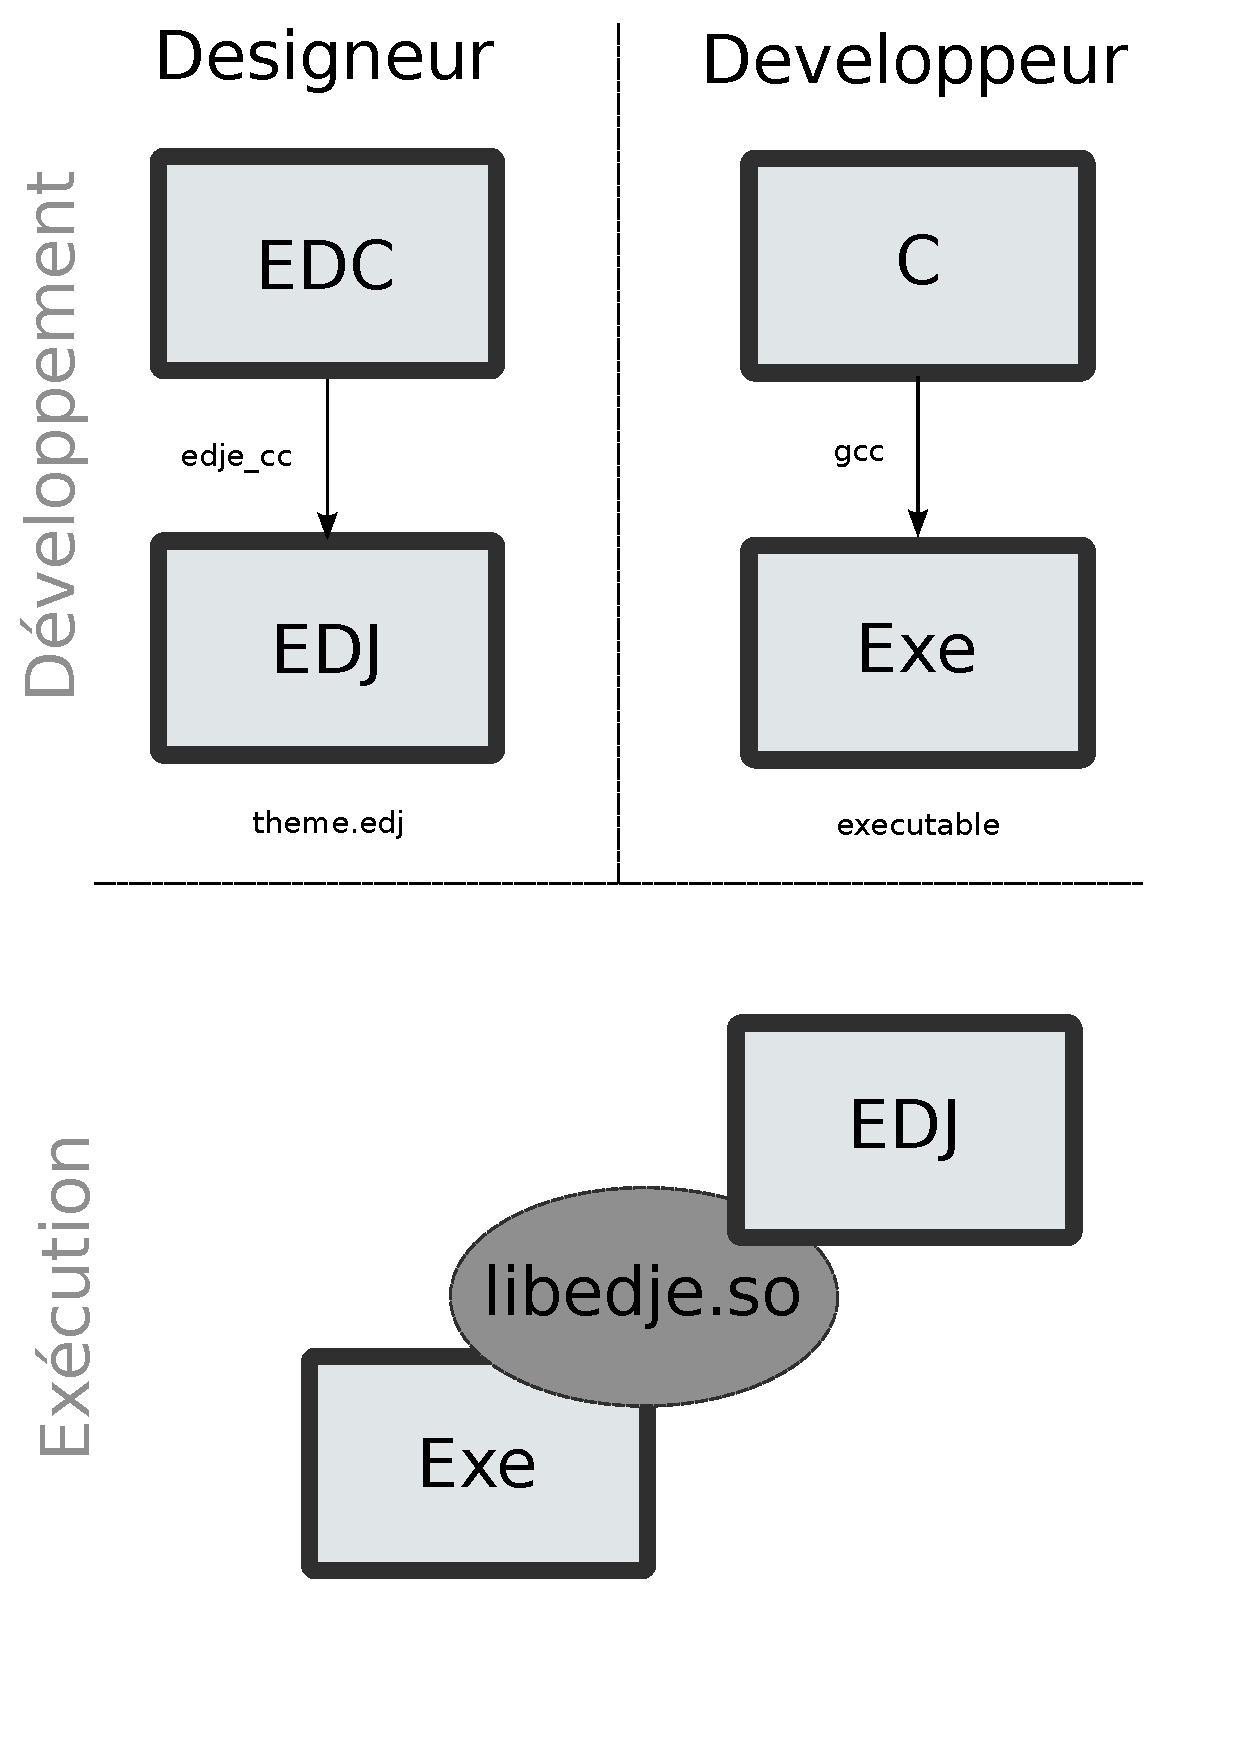
\includegraphics[scale=0.7]{images/workflow.pdf}
  \end{center}
  \caption{Edje Workflow}
\end{figure}

\section{Les Bases}
Dans ce chapitres, nous allons voir les bases du language de description EDC.

Une fichier EDC (Edje Data Collection) minimal ressemble a ceci : (fichier
tut01/tut01.edc)

\begin{lstlisting}[language=c]
 collections {
   group {
      name: "interface";
      parts {
         /* Rectangle Rouge */
         part {
            name: "Rectangle";
            type: RECT;
            description {
               state: "default" 0.0;
               color: 255 0 0 255;
            }
         }
      }
   }
}
\end{lstlisting}

Nous pouvons voir dans cette exemple le mot clef ``collection'' qui comme son
nom l'indique est un ensemble de ``groupes''.
Dans cette exemple nous avons un seul groupe, nommée ``interface''.
Un groupe est lui meme un ensemble, et représente un objet, qui pourra être
manipulé sur le canvas graphique plus tard dans notre programme ou réutilisé
dans le fichier edc.
Un Group contient des ``parts'' qui sont les primitives que sais manipuler Evas.
Voici une liste exhaustive des ``parts'' que nous pouvons utiliser :
\begin{itemize}
\item Les rectangles : RECT;
\item Les images : IMAGE;
\item Les textes : TEXT;
\item Les blocs de texte : TEXTBLOCK;
\item Les containers : SWALLOW;
\item Les groupes : GROUP;
\item Les boites : BOX;
\item Les tables : TABLE;
\item Les objects externes : EXTERNAL;
\end{itemize}
Chaque type fera l'objet d'une étude plus approfondie dans la suite de ce
tutoriel.

Dans notre exemple nous décrivons donc un Rectangle rouge, rien de bien
original. Nous allons maintenant compiler ce fichier edc en un fichier binaire
EDJ.  :

\begin{lstlisting}
edje_cc tut01.edc
\end{lstlisting}

Si tout c'est bien passé, nous devrions trouver un fichier tut01.edj dans notre
répertoire. Comme nous l'avons vu un peu plus haut. Ce fichier edj doit être
chargé par notre programme pour pouvoir être affiché. Dans un premier temps nous
allons donc utiliser un outil tres pratique proposé par edje : edje\_player.

\begin{lstlisting}
edje_player tut01.edc
\end{lstlisting}

Et voici le résultat : Un Rectangle Rouge affiché a l'écran ! Emotionnelement
intense.
Que ceux qui n'ont pas la cher de poule a ce moment précis arrêtent tout de
suite la lecture. Quand aux autres, vous pouvez trouver ci-dessous une capture
d'écran de l'interface que nous allons développer dans la suite de ce tutoriel.
j'ai choisis le développement d'un interface (tactile) simple, qui nous
permettra d'apprehender les différents concept de Edje par la pratique.

Voici le résultat final:
\begin{figure}
  \begin{center}
    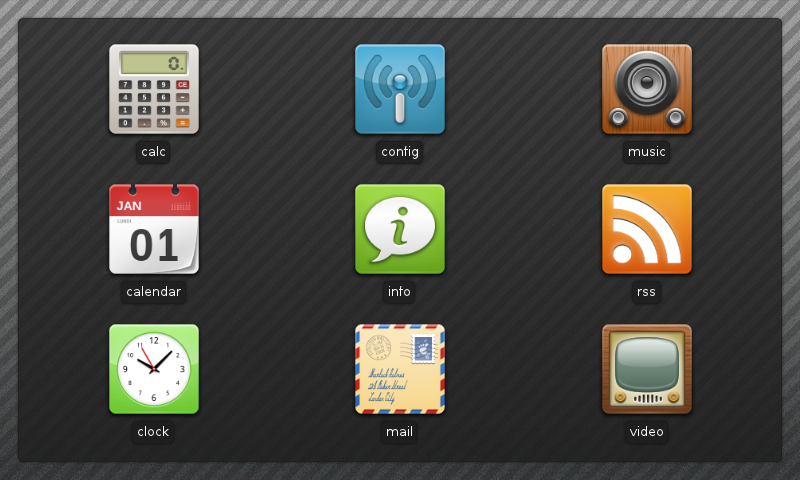
\includegraphics[scale=0.5]{images/screenshot1.png}
  \end{center}
  \caption{Interface edje à la fin de ce tutoriel}
\end{figure}

\section{Les Images}
\subsection{Les parts de type IMAGE}
Les explication de cette section portent sur le fichier
\href{file://tut02/tut02.edc}{tut02/tut02.edc}.

En partant du premier exemple, nous allons ajouter un fichier qui sera le fond
de notre interface.

Edje supporte un large type d'images, celles supportées par Evas,
PNG, JPEG, TIFF, BMP, ...
Pour décrire une image, il faut créer un part de type ``IMAGE''.
Et dire a edje quelle image insérer :

\begin{lstlisting}
 part {
   name: "Fond";
   type: IMAGE;
   description {
     state: "default" 0.0;
     image.normal: "bg.jpg";
   }
 }
\end{lstlisting}
\subsection{la directive images}
Comme nous avons vu précédement, le fichier EDJ généré contient toutes les
ressources de notre interface, images incluses. Si nous compilons avec edje\_cc
ce fichier, ``bg.jpg'' ne sera pas trouvé dans nos ressources. Il faut ajouter
cette images dans la collection. Ceci est réalisé par l'ajout de cette directive
:
\begin{lstlisting}
   images {
      image: "bg.jpg" COMP;
   }
\end{lstlisting}

A quoi correspond ``COMP''. Edje ajoute les images dans le fichier binaire EDJ,
et nous pouvons lui dire de compresser ou non cette image.
Plusieurs type de compressions sont supportés :
\begin{itemize}
\item RAW: Uncompressed.
\item COMP: compression sans perte, comparable au format PNG.
\item LOSSY [0-100]: comression avec perte avec une qualité pouvant allé
de 0 à 100, comparable au format JPEG
\item USER: l'image n'est pas intégrée au fichier edje, mais est lue depuis
le disque.
\end{itemize}

Attention cependant, si vous utilisez la balise RAW, a la taille
finale de votre fichier binaire.
Pour une image de 800x600 en 32bits de couleurs (RGBA), la taille embarqué dans
le fichier binaire sera : 800x600x4 ~= 1.8MO !

\subsection{edje\_cc et les images}
Le compilateur edje cherche les images dans les repertoires relativement au
repertoire ou il est executé.
Nous avons la possibilité de donner l'emplacement relative dans nos fichiers
edc. Par exemple :

\begin{lstlisting}
   images {
      image: "images\bg.jpg" COMP;
   }
\end{lstlisting}

Ceci peut tres vite devenir rebarbatif et long a écrire, nous pouvons donc
ajouter les répertoires qui contiennent nos images en utilisant l'argument
``-id'' (image directory) de edje\_cc

\begin{lstlisting}
edje_cc -id images -id images\icons file.edc
\end{lstlisting}

Pour faciliter la compilation, vous trouverez dans le répertoire de ce tutorial,
un script shell qui permet de compiler tous les fichiers edc (et C dans la
suite) nommé build.sh

\begin{lstlisting}
.\build.sh #compile l'intégralite des exemples.
.\build.sh #tut02 compile l'exemple contenu dans le repertoire tut02
\end{lstlisting}

Les fichiers binaires sont quand a eux générés dans le répertoire build.

\subsection{Les motifs}
Edje permet également l'affichage de motifs a l'écran en répétant une images.
Le fichier \href{file://tut03/tut03.edc}{tut03/tut03.edc} montre comment
utiliser une image motif avec la balise fill
\begin{lstlisting}
 size {
   relative: 0.0 0.0;
   offset: 20 20;
 }
\end{lstlisting}

Dans notre cas l'image a une taille de 20x20px nous voulons qu'elle soit répétée
sur l'axe des X et des Y.

Il y a plusieurs autres options permettant de repeter les motifs, je vous laisse
les découvrir par vous même, tout est décris dans la
\href{http://docs.enlightenment.org/auto/edje/edcref.html}[documentation de edje]


\section{Le Texte}
\subsection{description d'une icone}
Regardons le code du fichier \href{file://tut04/tut04.edc}{tut04/tut04.edc} plus
en détails. Un nouveau groupe a été ajouté nommée ``icon''. Il contient une
image ``icon.png'' et un nouveau part de type ``TEXT''.

\begin{lstlisting}
  part {
    name: "text";
    type: TEXT;
    description {
      state: "default" 0.0;
      color: 0 0 0 255;
      text {
        font: "Sans";
        size: 12;
        text: "Description";
      }
    }
  }
\end{lstlisting}

Les différentes options parlent d'elle méme :
\begin{itemize}
\item Couleur du texte : Noir;
\item Fonte utilisée ``Sans'';
\item Taille de la fonte : 12;
\item Texte a afficher ``Description'';
\end{itemize}

Regardons a quoi ressemble notre exemple avec edje\_player. Attention dans cet
exemple nous avons deux groupes. Nous devons donc spécifier a ejde\_player quel
groupe nous voulons visualiser, et nous allons également lui dire de changer la
couleur de fond.

\begin{lstlisting}
edje_player -c=255,255,255,255 -g icon tut04.edj
\end{lstlisting}

Nous sommes loins du résultat escompté ! Par défaut tous les parts sont
centrés au centre de l'écran et occupe tout le taille du groupe. Nous devons
décrire comment les objets sont placés les uns par rapport aux autres.
C'est l'objet des tutoriaux 5 à 8.


\section{Placement des objets}
\subsection{Proportions}

L'icône se doit d'être carré, c'est le cas de toutes les icônes en informatique
non ?  Pour cela Edje propose la balise aspect et aspect preference. Ces deux
balises sont liés. Regardons a quoi ca ressemble pour un définir un part carré:
\begin{lstlisting}
  aspect: 1.0 1.0;
  aspect_preference: BOTH;
\end{lstlisting}

aspect prends deux flottants comme paramétres, min et max. Dans un cas normal,
les dimensions de l'objet ne sont pas liés, en utilisant le paramétre aspect,
on force edje a garder un ration entre la largeur et la hauteur de notre part.
Dans le cas 1.0 1.0 l'icône aura donc meme hauteur et largeur.
aspect\_preference, lui donne la direction on veux que ce ration s'applique.
Rien de mieux pour comprendre qu'un exemple. regardez les fichier tut05.1.edj,
tut05.2.edj et tut05.3.edj pour visualiser les effets de aspect et
aspect\_preference

\subsection{Positions relatives et offset}

Edje permet de positionner les objets les uns par rapport aux autres de deux
façons. Positionnement relatifs et positionnement absolu.

Le positionnement relatif est en pourcent (valeur ramenée a un floatant entre
0.0 et 1.0) alors que les positions absolu sont en pixels.

Les balises rel1 et rel2 permettent de donner la position d'un objet par rapport
à un autre. Par défaut la position est celle par rapport au groupe.
Le positionnement relatif est donnée avec la balise rel1.relative et
rel2.relative alors que le positionnement absolu est donnée par rel1.offset et
rel2.offset.

\begin{figure}
  \begin{center}
    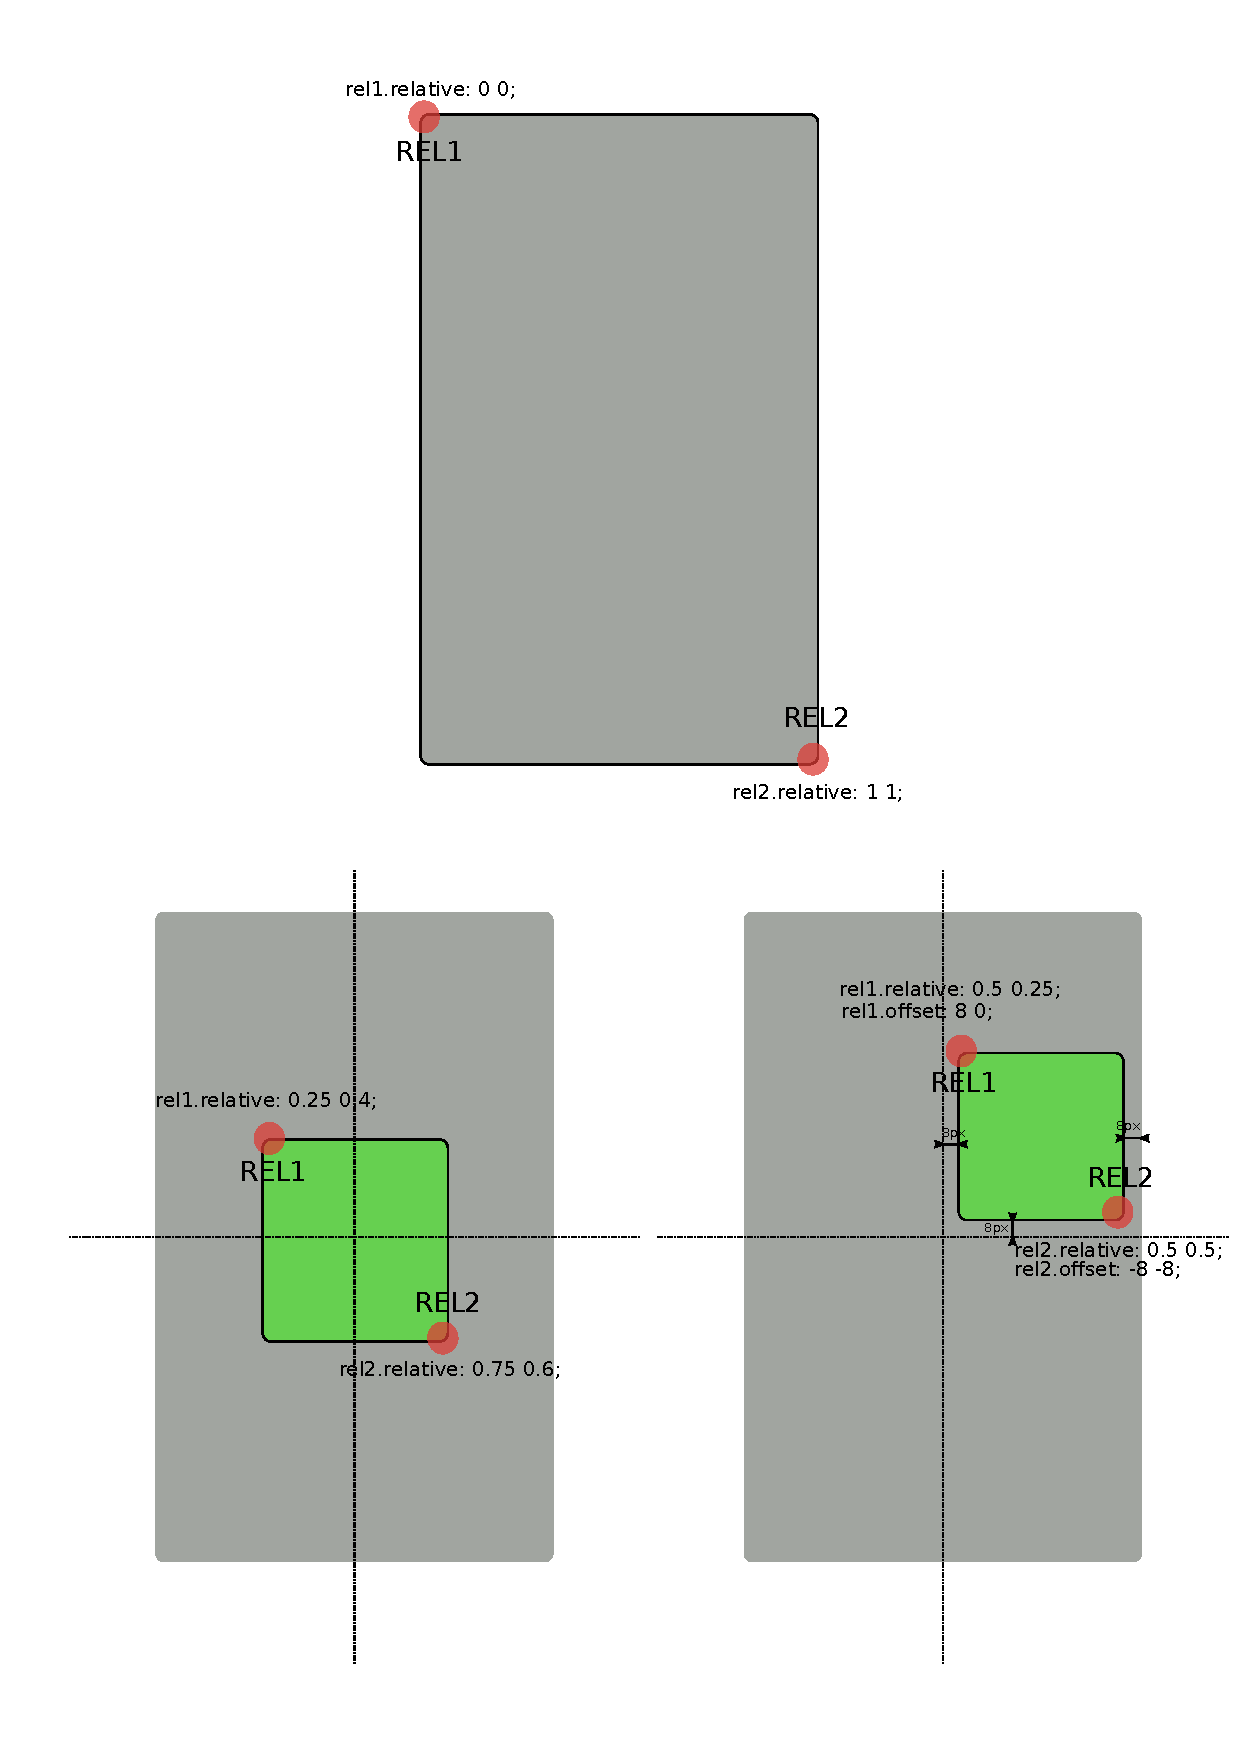
\includegraphics[scale=0.7]{images/rel1rel2.pdf}
  \end{center}
  \caption{Positionnement relatif et absolu}
\end{figure}

Dans cet exemple le positionnement est relatif au groupes, mais nous pouvons
spécifier un positonnement par rapport à un autre part en utilisant la balise :

\begin{lstlisting}
rel1.to: "autre_part1";
rel1.to: "autre_part2";
\end{lstlisting}

Ou encore relativement à un autre part mais uniquement sur un l'axe X ou Y :
\begin{lstlisting}
rel1.to_x: "autre_part1";
rel1.to_y: "autre_part2";
\end{lstlisting}


Pour l'exemple du fichier tut06.edc, j'ai choisis depositionner le texte en bas
du groupe. Le texte pouvant être dynamique, comme nous allons voir plus loin,
nous pouvons demander a Edje de calculer sa taille, c'est le role de
\begin{lstlisting}
min:: 1 1;
\end{lstlisting}

Edje vas calculer la  hauteur et la largeur du texte en fonction de la police,
et le part aura donc cette taile. Il nous reste plus qu'ensuite a positionner
l'icone au dessus de ce texte (balise rel2.to: \"texte\")
On ajoute également un bordure de 8 pixels autour de l'icone pour plus de
lisibilité.
\begin{lstlisting}
  rel1.relative: 0 0;
  rel1.offset: 8 8;
  rel2.relative: 1 0;
  rel2.offset: -7 -7;
  rel2.to: "text";
\end{lstlisting}

Vous verrez également une telle description sous cette forme :
\begin{lstlisting}
  rel1 {
    relative: 0 0;
    offset: 8 8;
  }
  rel2 {
    relative: 1 0;
    offset: -7 -7;
    to: "text";
  }
\end{lstlisting}

Ces deux notations sont entiérement identiques.

\section{Images bordurées}

Nous arrivons ici a une des fonctionalités que je préfére dans edje ! les
bordures (borders en anglais). Ca tient en une ligne, mais ca rends de grands
services.

\begin{lstlisting}
image.border: 8 8 8 8;
\end{lstlisting}

C'est spécifique aux parts de type ``IMAGES''. Cette ligne impose a Edje de ne
redimensionner toutes les parties de l'image, sauf les bordures. Le cas se
présente souvent lorsque on utilise une image avec des coins arrondis par
exemples, comme c'est le cas avec le contour du texte.

les paramétres de cette balise sont les suivants left, right, top, width et les
parmétres sont donnés en pixels.

\begin{figure}
  \begin{center}
    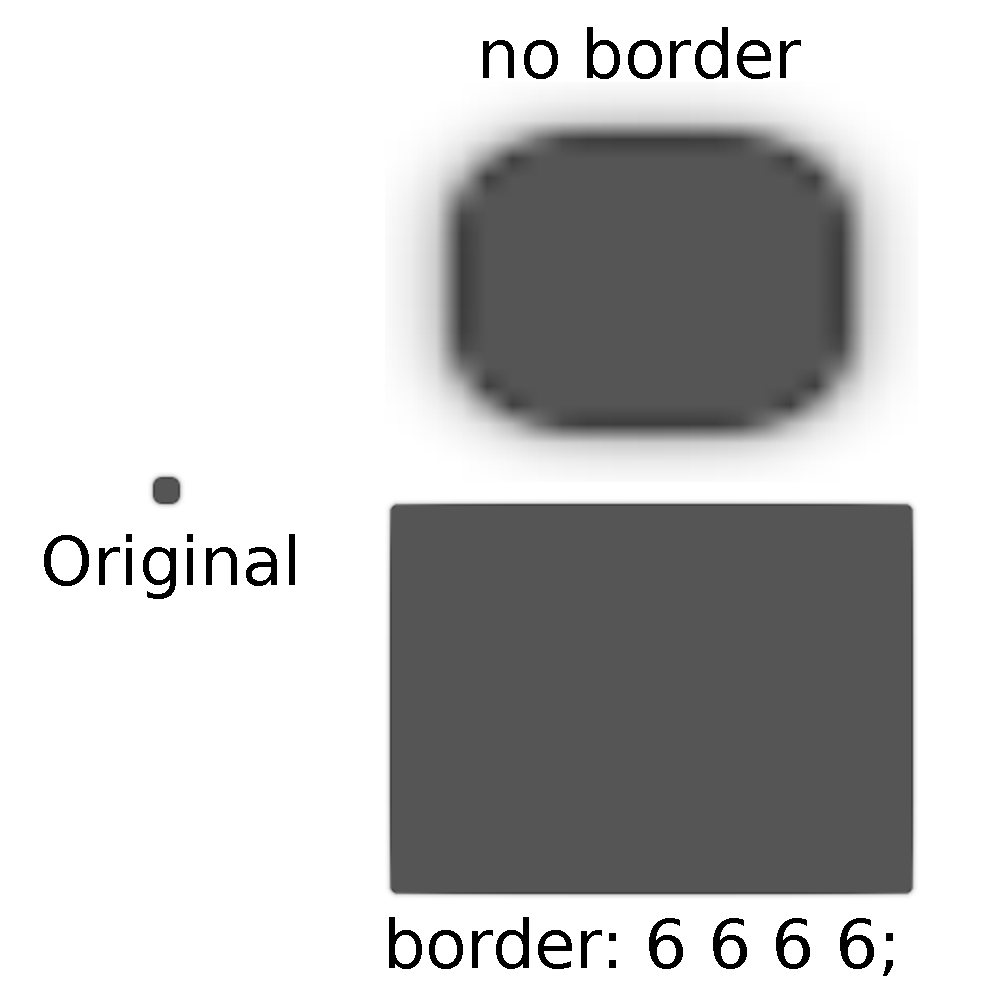
\includegraphics[scale=0.5]{images/border_diff.pdf}
  \end{center}
  \caption{Avec et sans bordure}
\end{figure}


\begin{figure}
  \begin{center}
    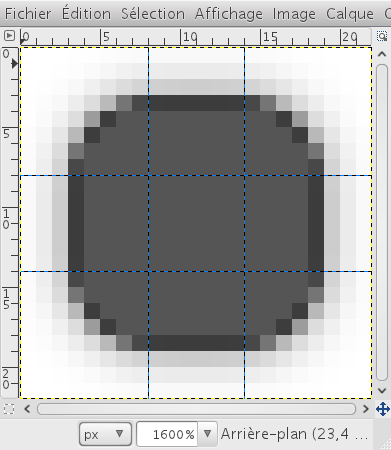
\includegraphics[scale=0.5]{images/border2.png}
  \end{center}
  \caption{Gimp et bordures}
\end{figure}



\section{Les programmes}

\subsection{Evenements souris}

Pour nous simplifier la vie par la suite, j'ai ajouté dans le fichier tut09
un part que j'ai nommé ``events'', qui se place au dessus de tous les autres
parts. L'ordre des parts est fonction de la position de la description dans le
groupe. C'est a dire que le part le plus bas dans le fichier est le plus haut
dans l'interface.

Ce part ``events'' semble ne servir a rien, puisqu'il a une transparence à 0,
mais il va nous rendre de grand service. Dans la suite il va nous permettre de
capturer tous les évenements souris de notre icone.

La balise visible indique a Edje si le part doit être affiché ou pas à l'écran
quelque soit la position, la taille ou toute autre propriétée du part.
Par défaut les parts sont visibles, mais parfois, nous pouvons faire en sorte
qu'un part devienne invisible. Nous voudrions par exemple a moment donné que
les évenements souris ne soient pas capturés, Il nous suffirait dont de mettre
cette propriété a 0 pour que plus aucun evenements ne soient traités pour ce
part.

\subsection{Les Programmes}

Un programme est une action que Edje va réaliser. Cela peut être de différents
types, un événement souris sur notre groupe, une signal provenant du programme
qui manipule notre groupe, un signal envoyé par un autre programme, un signal
envoyé par edje.

Le fichier tut10.edc présente un exemple de programme qui réagit a un événement
bouton 1 de la souris enfoncé :

\begin{lstlisting}
  program {
    name: "mouse_down";
    signal: "mouse,down,1";
    source: "events";
    action: STATE_SET "down" 0.0;
    target: "icon";
  }
\end{lstlisting}

A quoi correspondent les différentes balises :

\begin{itemize}
\item name: C'est le nom du programme
\item signal: c'est la chaine de caractére qui défiini le signal reçu, dans ce
cas c'est un signal envoyé par edje lorsque le bouton 1 de la souris est enfoncé
sur le part défini dans la balise ``source''.
\item source le part qui est responsable  du signal. La souris doit être enfoncé sur ce
part. On voit ici que ce part nous sert a quelque chose ! Si il n'existait pas
nous aurions du dupliquer ce programme pour réaliser l'action sur le part icon,
texte et texte_bg !
\item action: L'action a réalisée lorsque le signal est reçu. Ici nous demandons
a Edje de changer l'état du part défini dans la balise ``target'' à "down" 0.0
\end{itemize}

Un part avoir plusieurs états, si il existe plusieurs description de celui-ci
C'est le role de la balise ``description'' que nous avons rencontrée mais pas
encore expliquée.

Tous les paramétres d'un part que nous avons vu jusqu'à présente : couleur,
alignement, la fonte ou la taille pour un texte, .... peuvent avoir différentes
valeurs d'une description a une autre.

\begin{lstlisting}
state: "default" 0.0;
\end{lstlisting}

Ce balise permet de donner un nom a notre état, ainsi qu'une flotant.
Revenons a notre exemple :

\begin{lstlisting}
  part {
    name: "icon";
    type: IMAGE;
    mouse_events: 0;
    description {
      state: "default" 0.0;
      aspect: 1.0 1.0;
      aspect_preference: BOTH;
      image.normal: "icon.png";
      rel1.relative: 0 0;
      rel1.offset: 8 8;
      rel2.relative: 1 0;
      rel2.offset: -7 -7;
      rel2.to_y: "text";
      align: 0.5 0.5;
    }
    description {
      state: "down" 0.0;
      inherit: "default" 0.0;
      color: 255 255 255 128;
    }
  }
\end{lstlisting}

Ici nous avons deux états : \"default\" 0.0 et \"down\" 0.0.
L'état down, hérite de toutes les propriétés de default sauf pour la couleur, ou
nous changeons l'alpha.

Couplé au programme précédent, cela aura pour effet de changer la transparence
lors d'un clic sur l'icone.

Nous pouvons vérifier ceci avec edje\_player :
\begin{lstlisting}
edje\_player tut10.edj -g icon
\end{lstlisting}



\end{document}

